% Name: Translation by a vector
% Description: Triangle ABC slid by the vector (4, −2): every point moves the same distance in the same direction, so the image A′B′C′ is congruent and keeps its orientation.
% Tags: transformation, translation, vector, coordinate geometry

\usetikzlibrary{arrows.meta}

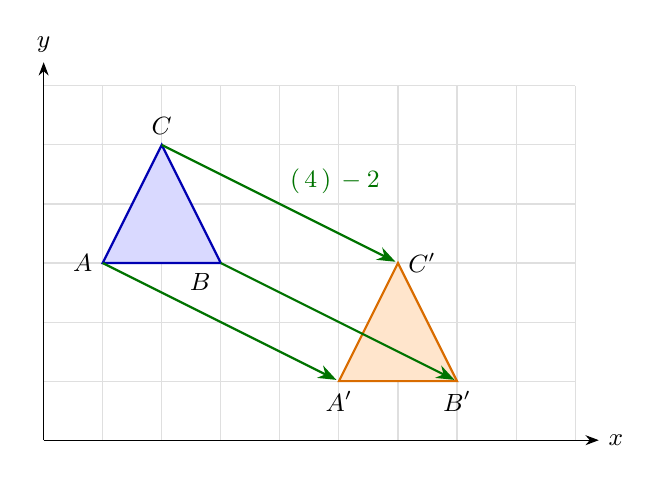
\begin{tikzpicture}[>={Stealth}, scale=0.75, every node/.style={font=\small}]
  % (x, y) maps to (x + 4, y - 2)
  \draw[gray!25] (0,0) grid (9,6);
  \draw[->] (0,0) -- (9.4,0) node[right] {$x$};
  \draw[->] (0,0) -- (0,6.4) node[above] {$y$};
  \draw[thick, fill=blue!15, draw=blue!70!black] (1,3) node[left] {$A$} -- (3,3) node[below left] {$B$} -- (2,5) node[above] {$C$} -- cycle;
  \draw[thick, fill=orange!20, draw=orange!85!black] (5,1) node[below] {$A'$} -- (7,1) node[below] {$B'$} -- (6,3) node[right] {$C'$} -- cycle;
  \draw[->, thick, green!45!black, shorten >=1pt] (1,3) -- (5,1);
  \draw[->, thick, green!45!black, shorten >=1pt] (3,3) -- (7,1);
  \draw[->, thick, green!45!black, shorten >=1pt] (2,5) -- node[above right] {$\begin{pmatrix} 4 \\ -2 \end{pmatrix}$} (6,3);
\end{tikzpicture}
